\documentclass[tikz,border=2pt]{standalone}
\usepackage[T1]{fontenc}
\usepackage{mathpazo}
\usepackage[scaled=.90]{helvet}
\usepackage{amsmath,amssymb}
\usetikzlibrary{arrows.meta,calc}

% Restrained editorial palette
\definecolor{paper}{HTML}{FFFFFF}
\definecolor{ink}{HTML}{222831}
\definecolor{midnight}{HTML}{223A5E}
\definecolor{petrol}{HTML}{3F7776}
\definecolor{aubergine}{HTML}{765B73}
\definecolor{steel}{HTML}{55718F}
\definecolor{copper}{HTML}{A8784A}
\definecolor{secondary}{HTML}{68727D}
\definecolor{hairline}{HTML}{C8CDD1}

\tikzset{
  hair/.style={draw=hairline,line width=.34pt},
  strongrule/.style={draw=midnight,line width=.56pt},
  architecture/.style={draw=ink,line width=.45pt},
  archdot/.style={circle,draw=ink,fill=paper,line width=.45pt,
                  minimum size=4.1pt,inner sep=0pt},
  every node/.style={text=ink}
}

\newcommand{\sectionfont}{\bfseries\fontsize{13.2}{14.2}\selectfont}
\newcommand{\titlefont}{\bfseries\fontsize{16.0}{17.2}\selectfont}
\newcommand{\methodfont}{\bfseries\fontsize{10.7}{11.6}\selectfont}
\newcommand{\bodyfont}{\fontsize{8.45}{9.7}\selectfont}
\newcommand{\metafont}{\fontsize{7.4}{8.3}\selectfont}
\newcommand{\labelfont}{\sffamily\bfseries\fontsize{5.4}{6.1}\selectfont}
\newcommand{\outcomefont}{\bfseries\fontsize{10.2}{11}\selectfont}
\newcommand{\timelinefont}{\fontsize{7.0}{8.1}\selectfont}

% Row label and value. The label x coordinate is #1, value x coordinate #2,
% baseline y coordinate #3, label text #4, value text #5.
\newcommand{\inforow}[5]{%
  \node[anchor=west,font=\labelfont,text=midnight] at (#1,#3) {#4};
  \node[anchor=west,font=\bodyfont] at (#2,#3) {#5};
}

\begin{document}
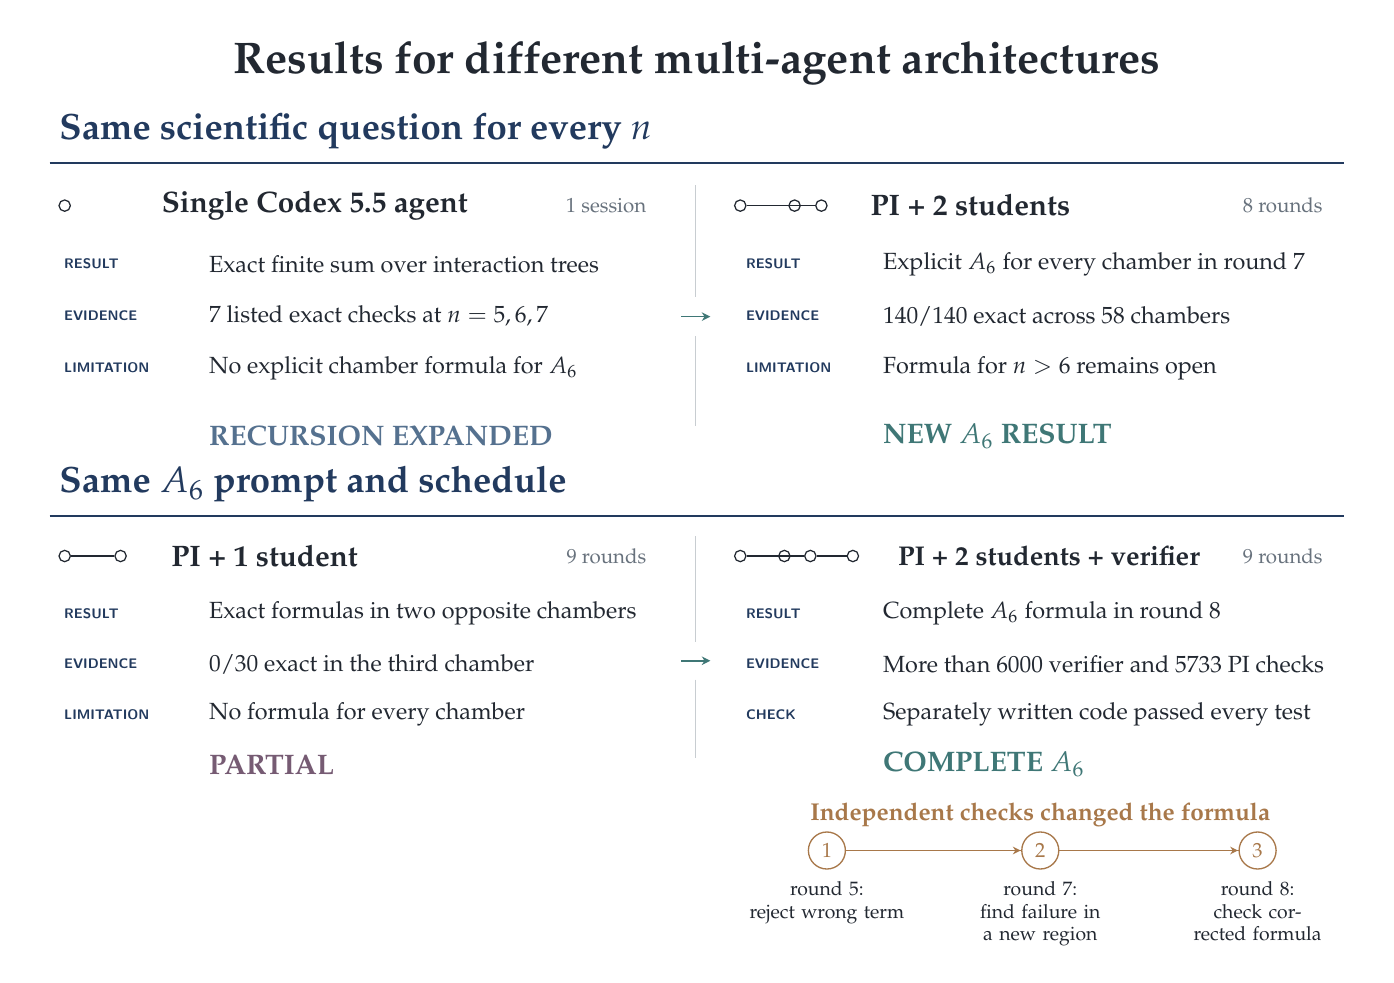
\begin{tikzpicture}[x=1cm,y=1cm]
  \fill[paper] (0,0) rectangle (17.0,11.62);

  \node[anchor=center,font=\titlefont,text=ink] at (8.50,11.16)
    {Results for different multi-agent architectures};

  % ======================== TOP COMPARISON BAND ========================
  \node[anchor=west,font=\sectionfont,text=midnight] at (.28,10.30)
    {Same scientific question for every $n$};
  %\node[anchor=east,font=\itshape\metafont,text=secondary] at (16.72,10.30)
  %  {models and total calls differ};
  \draw[strongrule] (.28,9.90)--(16.72,9.90);

  % Left method header: one agent
  \node[archdot] at (.47,9.36) {};
  \node[anchor=west,font=\methodfont] at (1.58,9.36)
    {Single Codex 5.5 agent};
  \node[anchor=east,font=\metafont,text=secondary] at (7.98,9.36)
    {1 session};

  % Right method header: PI plus two students
  \node[archdot] (tpi) at (9.05,9.36) {};
  \node[archdot] (tsone) at (9.74,9.36) {};
  \node[archdot] (tstwo) at (10.08,9.36) {};
  \draw[architecture] (tpi)--(9.48,9.36);
  \draw[architecture] (9.48,9.36)--(tsone);
  \draw[architecture] (9.48,9.36)--(tstwo);
  \node[anchor=west,font=\methodfont] at (10.58,9.36)
    {PI + 2 students};
  \node[anchor=east,font=\metafont,text=secondary] at (16.57,9.36)
    {8 rounds};

  % Top-band rows
  \inforow{.34}{2.18}{8.62}{RESULT}{Exact finite sum over interaction trees}
  \inforow{.34}{2.18}{7.96}{EVIDENCE}{7 listed exact checks at $n=5,6,7$}
  \inforow{.34}{2.18}{7.30}{LIMITATION}{No explicit chamber formula for $A_6$}

  \inforow{9.00}{10.74}{8.62}{RESULT}{Explicit $A_6$ for every chamber in round 7}
  \inforow{9.00}{10.74}{7.96}{EVIDENCE}{140/140 exact across 58 chambers}
  \inforow{9.00}{10.74}{7.30}{LIMITATION}{Formula for $n>6$ remains open}

  % Central separator and richer-architecture cue
  \draw[hair] (8.48,9.62)--(8.48,8.20);
  \draw[hair] (8.48,7.70)--(8.48,6.56);
  \draw[-{Stealth[length=3.1pt,width=3.1pt]},petrol,line width=.56pt]
    (8.30,7.95)--(8.67,7.95);

  % Top outcomes
  \node[anchor=west,font=\outcomefont,text=steel] at (2.18,6.43)
    {RECURSION EXPANDED};
  \node[anchor=west,font=\outcomefont,text=petrol] at (10.74,6.43)
    {NEW $A_6$ RESULT};

  % ======================= SECOND COMPARISON BAND ======================
  \node[anchor=west,font=\sectionfont,text=midnight] at (.28,5.82)
    {Same $A_6$ prompt and schedule};
  %\node[anchor=east,font=\itshape\metafont,text=secondary] at (16.72,5.82)
  %  {same agent models; team on the right uses more calls};
  \draw[strongrule] (.28,5.42)--(16.72,5.42);

  % Left method header: PI plus one student
  \node[archdot] (bpi) at (.47,4.91) {};
  \node[archdot] (bs) at (1.18,4.91) {};
  \draw[architecture] (bpi)--(bs);
  \node[anchor=west,font=\methodfont] at (1.70,4.91)
    {PI + 1 student};
  \node[anchor=east,font=\metafont,text=secondary] at (7.98,4.91)
    {9 rounds};

  % Right method header: PI plus two students and a verifier
  \node[archdot] (vpi) at (9.05,4.91) {};
  \node[archdot] (vsone) at (9.61,4.91) {};
  \node[archdot] (vstwo) at (9.94,4.91) {};
  \node[archdot] (ver) at (10.48,4.91) {};
  \draw[architecture] (vpi)--(9.40,4.91);
  \draw[architecture] (9.40,4.91)--(vsone);
  \draw[architecture] (9.40,4.91)--(vstwo);
  \draw[architecture] (vstwo)--(ver);
  \node[anchor=west,font=\bfseries\fontsize{9.8}{10.6}\selectfont] at (10.93,4.91)
    {PI + 2 students + verifier};
  \node[anchor=east,font=\metafont,text=secondary] at (16.57,4.91)
    {9 rounds};

  % Second-band rows
  \inforow{.34}{2.18}{4.18}{RESULT}{Exact formulas in two opposite chambers}
  \inforow{.34}{2.18}{3.54}{EVIDENCE}{0/30 exact in the third chamber}
  \inforow{.34}{2.18}{2.90}{LIMITATION}{No formula for every chamber}

  \inforow{9.00}{10.74}{4.18}{RESULT}{Complete $A_6$ formula in round 8}
  \inforow{9.00}{10.74}{3.54}{EVIDENCE}{More than 6000 verifier and 5733 PI checks}
  \inforow{9.00}{10.74}{2.90}{CHECK}{Separately written code passed every test}

  % Central separator and richer-architecture cue
  \draw[hair] (8.48,5.16)--(8.48,3.82);
  \draw[hair] (8.48,3.34)--(8.48,2.35);
  \draw[-{Stealth[length=3.1pt,width=3.1pt]},petrol,line width=.56pt]
    (8.30,3.58)--(8.67,3.58);

  % Second outcomes
  \node[anchor=west,font=\outcomefont,text=aubergine] at (2.18,2.26)
    {PARTIAL};
  \node[anchor=west,font=\outcomefont,text=petrol] at (10.74,2.26)
    {COMPLETE $A_6$};

  % ===== VERIFIER TIMELINE: belongs only to PI + 2 students + verifier =====
  \node[anchor=center,font=\bfseries\fontsize{8.8}{9.6}\selectfont,text=copper]
    at (12.86,1.62) {Independent checks changed the formula};
  \draw[copper,line width=.46pt] (10.15,1.17)--(15.62,1.17);

  \foreach \x/\num in {10.15/1,12.86/2,15.62/3}{
    \node[circle,draw=copper,fill=paper,text=copper,line width=.48pt,
          minimum size=4.7mm,inner sep=0pt,font=\metafont] at (\x,1.17) {\num};
  }
  \draw[-{Stealth[length=2.8pt,width=2.8pt]},copper,line width=.46pt]
    (10.39,1.17)--(12.61,1.17);
  \draw[-{Stealth[length=2.8pt,width=2.8pt]},copper,line width=.46pt]
    (13.10,1.17)--(15.37,1.17);

  \node[anchor=north,align=center,text width=2.35cm,font=\timelinefont] at (10.15,.90)
    {round 5:\\reject wrong term};
  \node[anchor=north,align=center,text width=2.35cm,font=\timelinefont] at (12.86,.90)
    {round 7:\\find failure in a new region};
  \node[anchor=north,align=center,text width=2.35cm,font=\timelinefont] at (15.62,.90)
    {round 8:\\check corrected formula};
\end{tikzpicture}
\end{document}
